\section{Effect of Access Strategy} \label{sec:res-access}

In section \ref{sec:optimizations}, we discussed various optimizations for accessing such grids in a stencil application. Here, we compare the performance of these approaches. Figure \ref{fig:storage-access} gives an overview of the possible storage/access-combinations.

\begin{figure}
	%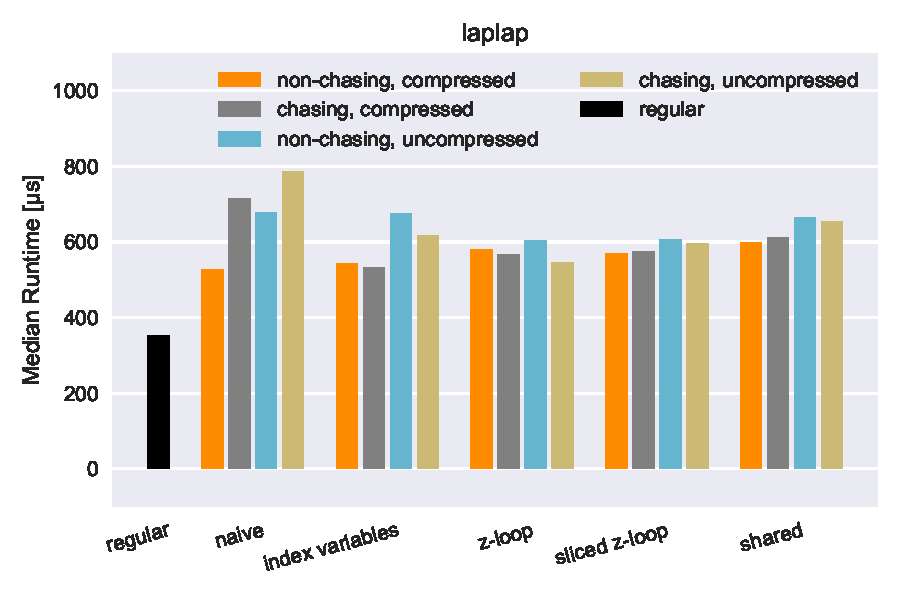
\includegraphics[scale=0.75]{laplap-zcurves-grouped-variants.pdf} % ./plot.py -i results/ultimate.csv -p grouped --size $((512*512*64)) --bar-groups variant --color storage --marker storage --z-curves z-curves --stencil laplap --title "laplap" -o results/variants/laplap-zcurves-grouped-variants.pdf --exclude laplap-regular-naive --scale-max 1000
	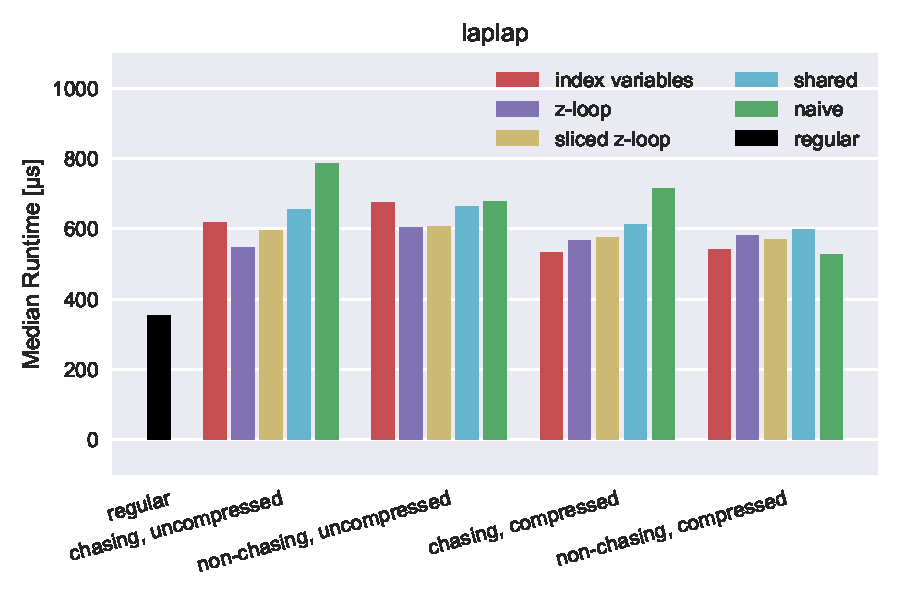
\includegraphics[scale=0.75]{laplap-zcurves-grouped-storage.pdf} % ./plot.py -i results/ultimate.csv -p grouped --size $((512*512*64)) --bar-groups storage --color variant --marker variant --z-curves z-curves --stencil laplap --title "laplap" -o results/variants/laplap-zcurves-grouped-storage.pdf --exclude laplap-regular-naive --scale-max 1000
	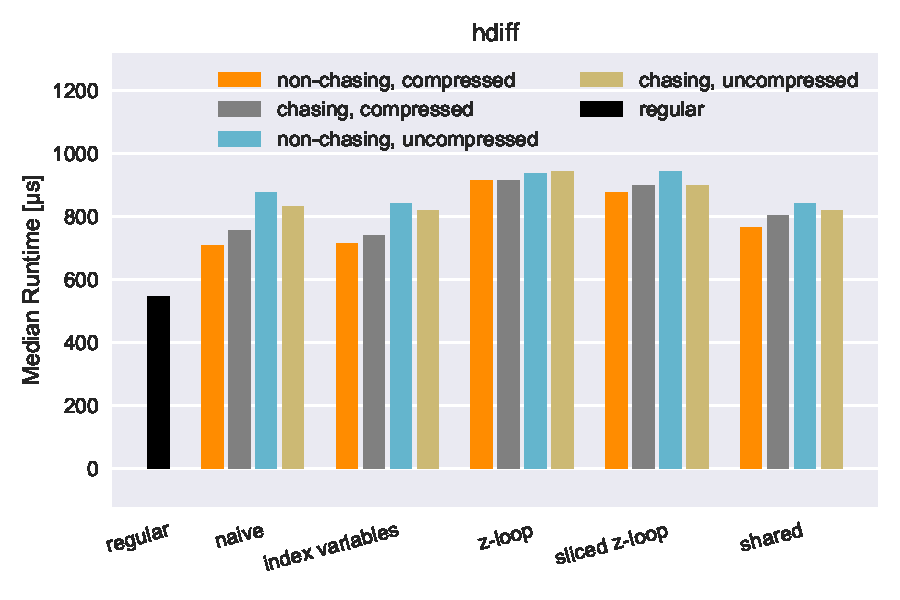
\includegraphics[scale=0.75]{hdiff-zcurves-grouped-variants.pdf} % ./plot.py -i results/ultimate.csv -p grouped --size $((512*512*64)) --bar-groups variant --color storage --marker storage --z-curves z-curves --stencil hdiff --title "hdiff" -o results/variants/hdiff-zcurves-grouped-variants.pdf --exclude hdiff-regular-naive --scale-max 1200
	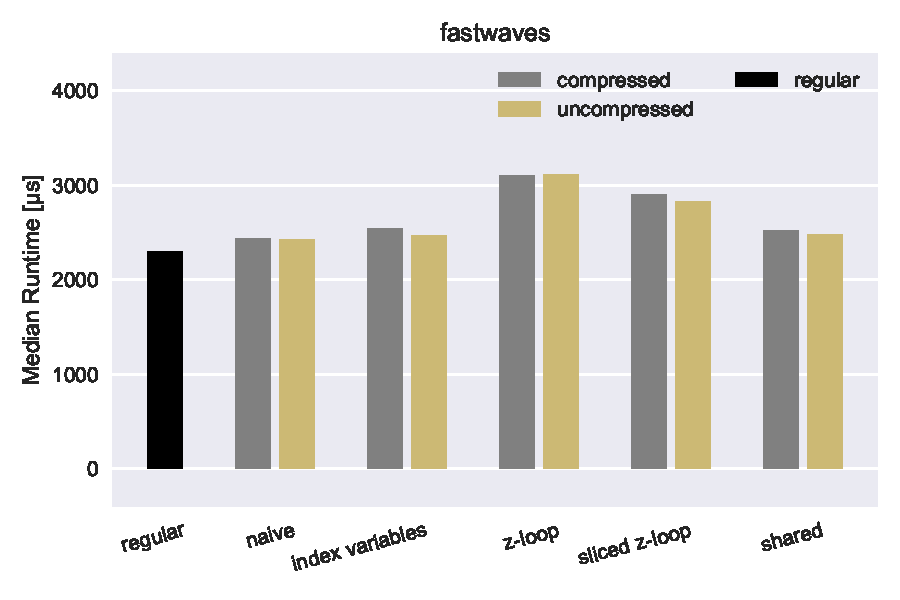
\includegraphics[scale=0.75]{fastwaves-zcurves-grouped-variants.pdf} % ./plot.py -i results/ultimate.csv -p grouped --size $((512*512*64)) --bar-groups variant --color storage --marker storage --z-curves z-curves --stencil fastwaves --title "fastwaves" -o results/variants/fastwaves-zcurves-grouped-variants.pdf --exclude fastwaves-regular-naive --scale-max 4000
	\caption{\label{fig:storage-access} Median runtimes across 20 runs for stencils on a $512\times512\times 64$-sized unstructured grid (z-curves layout). The fastest blocksize was chosen and reported per variant. The time reported for the regular grid is the fastest of all implemented regular variants. Results for row-major-stored grids are similar. Note that for the \emph{fastwaves} stencil, only direct neighbors are accessed; pointer chasing thus never occurs.}
\end{figure}

\subsection{\emph{Naive} and \emph{Idxvar} Access Strategies}
The \emph{naive} and \emph{idxvar} (index variables) access strategies are the fastest for all three stencils. In some cases, the \emph{naive} access strategy is faster than the \emph{idxvar} variant by a very slight margin. This is the case, for example, in the fastwaves stencil or the horizontal diffusion stencil executed on a non-chasing, compressed grid. This result might appear surprising at first, as the naive strategy repeatedly performs memory lookups for the same neighborship pointers. The index variables approach tries to reduce these reduntant lookups by storing the needed neighborship indices in temproary variables at the start of the kernel execution. However, this adds some overhead.

For one, the index variables variant for the fastwaves kernel leads to a higher register use when compiled (44 registers for \emph{idxvar} versus 42 for \emph{naive}). As registers are shared across threads of a block, this reduces the theoretical amount of threads that can be launched concurrently. As this difference is not present in the other stencils, this does not appear to be the main reason for the advantage, however. There are two more likely explanations for the advatnage of the \emph{naive} variant: First, access to the same memory location in the \emph{naive} kernel becomes as cheap as a register access after a neighborship pointer are read for the first time, as it will be held in the L1 cache. Reaccessing the same memory location helps keep the values fresh in all caches. As such, when a different thread requires the same memory location from the neighborship table, it is more likely to be in cache in the \emph{naive} variant. Second, the naive approach has better \emph{instruction level parallelism}. Because the index variables are assigned at the start of the \emph{idxvar} variant, all loads to the neighborship table are gathered in one sequence and must be executed before anything else. In the \emph{naive} approach, on the other hand, neighborship pointers are (re-)loaded only when needed in calculations. Thus, after one neighbor has been loaded, useful calculations using its value may already be performed. Table \ref{tab:fastwaves-naive-idxvar-metrics} details profiler metrics that support these claims.

\begin{table}
	\begin{tabular}{l l l}
		\hline
		Metric & \emph{naive} & \emph{idxvar} \\
		\hline
		Run time & $\mathbf{2438\mu s}$ & $2543\mu s$ \\
		Global load transactions & $126264460$ & $124235165$ \\
		L1 transactions & $38077396$ & $34593863$ \\
		L2 transactions & $56635611$ & $57264861$ \\
		Device Memory transactions & $36825619$ & $37327310$ \\
		Executed Instructions Per Cycle & $\textbf{0.522}$ & $0.497$ \\
		\hline
	\end{tabular}
	\caption{\label{tab:fastwaves-naive-idxvar-metrics}Selection of metrics for \emph{fastwaves} stencil run on a $512\times 512\times 1$-sized unstructured grid (z-curves layout, compressed neighborship table) with $32\times 1\times 8$ threads, which is the fastest block size for both variants. The \emph{naive} implementation is faster, even though it redoes the index lookups in the neighborship tables. The total global transaction count shows that the \emph{idxvar} variant successfully reduces the number of neighborship lookups performed. However, the cache transactions (L1 and L2) indicate that the naive variant keeps cache contents fresher and results in more cache hits. This is evidenced by the lower number of actual device memory reads in the naive approach, despite the idxvar approach requesting less memory.}
\end{table}

\subsection{\emph{Shared} Access Strategy}

\begin{verbatim}
% mention it is faster for no-chase, uncompressed grid storage
% -> explicit shared memory usage better than relying on cache when there is a very large number of neighbors

% TODO
% - shared is almost same as idxvar due to caches
% - overhead of synchronization makes it slightly slower
% - back this up with metrics
\end{verbatim}

\subsection{\emph{Z-loop} and \emph{Z-loop-sliced} Access Strategies}

\begin{verbatim}
% TODO
% - reiterate what the supposed advantage of z loop is
% - Why is it faster for uncompressed variants, why slower for compressed?
%    -> Back up with metrics!
\end{verbatim}
